\documentclass{article}
\usepackage{graphicx}
\usepackage{subcaption]
	\begin{document}
		\begin{figure}[h!]
			\centering
			\begin{subfigure}[b]{0.2\linewidth}
				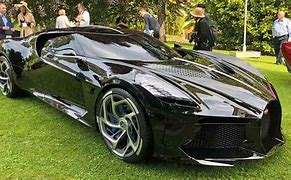
\includegraphics[width=\linewidth]{my car.jpg}
				\caption{my car}
			\end{subfigure}
		\begin{subfigure}[b]{0.2\linewidth}
		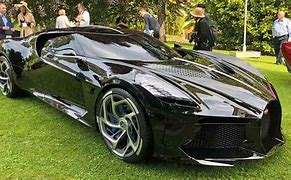
\includegraphics[width=\linewidth]{my car.jpg}
		\caption{more cars}
		\end{subfigure}
	\begin{subfigure}[b]{0.2\linewidth}
		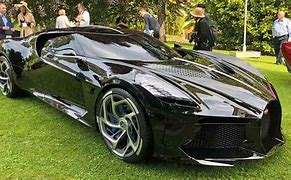
\includegraphics[width=\linewidth]{my car.jpg}
		\caption{such a splendid car}
		\end{subfigure}
		\begin{subfigure}[b]{0.5\linewidth}
			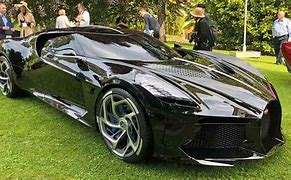
\includegraphics[width=\linewidth]{my car.jpg}
			\caption{wow}
			\end{subfigure}
		\caption{the same car, again and again}
		\label[fig:car]
	\end{figure}
\end{document}	